\chapter{Logica predicativa}
La logica dei predicati introduce, nello studio delle proposizioni, attributi di oggetti. In tale logica le proposizioni vengono analizzate in soggetto e predicato.

L’alfabeto di un linguaggio per la logica dei predicati si compone di:
\begin{enumerate}
    \item simboli per variabili, denotati da x, y, z...
    \item simboli per costanti, denotati da a, b, c...
    \item simboli funzionali a 1, 2,… posti (si dice di arità 1, 2...), denotati da f, g, h...
    \item simboli predicativi a 1, 2... posti, denotati da P(-), Q(-, -)...
    \item i connettivi, $\neg, \implies, \land, \lor, \iff$;
    \item i quantificatori $\forall, \exists$;
    \item parentesi e virgole.
\end{enumerate}

I \textbf{\textit{termini}} di un linguaggio per la logica dei predicati sono definiti come: 
\begin{itemize}
    \item variabili e costanti;
    \item se $t_1, ..., t_n$ sono termini ed f ha n posti, $f (t_1, ..., t_n)$ è un termine.
\end{itemize}

Le \textbf{\textit{formule}} sono espressioni del linguaggio definite come:
\begin{itemize}
    \item Se P ha n posti e $t_1, ..., t_n$ sono termini, $P (t_1, ..., t_n)$ è una formula (atomica);
    \item se A e B sono formule, lo sono anche $A, A \implies B, A \land B, A \lor B e A \iff B$;
    \item se A è una formula, lo sono anche $\forall x A$ e $\exists x A$, dove x è una variabile.
\end{itemize}

\begin{example}
Si formalizzino, usando il linguaggio presentato per il calcolo dei predicati, le seguenti frasi:
\begin{itemize}
    \item nessun uomo è mortale e padre di se stesso;
    \item il Sole è la stella più vicina alla Terra;
\end{itemize}

\textbf{Soluzione 1.}: Sia M(-) il predicato “essere mortale” e P (-,-) il predicato “essere padre di”. Allora, la precedente frase può essere formalizzate nel modo seguente:
\begin{equation*}
    \neg \exists x (M (x) \land P (x, x));
\end{equation*}

\textbf{Soluzione 2.}: Sia S(-) il predicato “essere stella” e V (-, -) il predicato “essere più vicino alla Terra di”; allora, la formula cercata è:
\begin{equation*}
    \forall x (S(x) \implies \lor (y, x))
\end{equation*}
dove y andrà interpretata con la costante Sol e (e ciò
chiuderà la formula).
\end{example}

\section{Regole per la costruzione di un tableau predicativo}
\begin{enumerate}
    \item se una formula di un ramo di un tableau è del tipo $\forall x A(x)$ oppure $\neg\exists x B(x)$, aggiungiamo un nuovo nodo:
    \begin{figure}[ht]
        \centering
        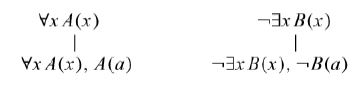
\includegraphics[width = 7cm]{images/rel_pred1.JPG}
    \end{figure}
    \item se una formula di un ramo di un tableau è del tipo $\exists x A(x)$ oppure $\neg\forall x B(x)$, aggiungiamo un nuovo nodo:
    \begin{figure}[ht]
        \centering
        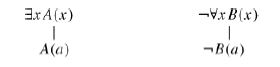
\includegraphics[width = 7cm]{images/rel_pred2.JPG}
    \end{figure}
    
\end{enumerate}

\begin{example}
Costruiamo il tableau predicativo per la negazione della
formula:

    $(\forall x P (x) \lor \forall x Q(x)) \implies \forall x (P (x) \lor Q(x))$
\begin{figure}[ht]
    \centering
    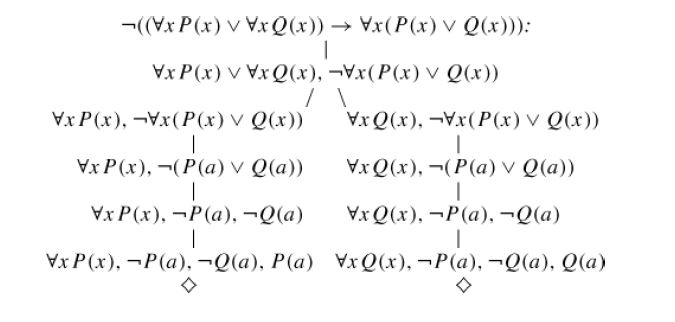
\includegraphics[width = 12cm]{images/es_tabl_pred.JPG}
\end{figure}

\end{example}